% /**
%  * A template for homework files in math classes. The 
%  * packages and newcommands are a good starting point.
%  *
%  * Author: James K. Pringle
%  * E-mail: jameskpringle@gmail.com
%  * Last Changed: 5 September 2013
%  *
%  * "LaTeX countains the increasing union of MS Word"
%  */
%~~~~~~~~~~~~~~~~~~~~~~~~~~~~~~~~~~~~~~~~~~~~~~~~~~~~~~~~~%
%%%%%%%%%%%%%%%%%%%%%%%%%%%%%%%%%%%%%%%%%%%%%%%%%%%%%%%%%%%
%                                                         %
%                        PAGE SETUP                       %
%                                                         %
%%%%%%%%%%%%%%%%%%%%%%%%%%%%%%%%%%%%%%%%%%%%%%%%%%%%%%%%%%%
\documentclass[letterpaper, 12pt]{article}\usepackage[]{graphicx}\usepackage[]{color}
%% maxwidth is the original width if it is less than linewidth
%% otherwise use linewidth (to make sure the graphics do not exceed the margin)
\makeatletter
\def\maxwidth{ %
  \ifdim\Gin@nat@width>\linewidth
    \linewidth
  \else
    \Gin@nat@width
  \fi
}
\makeatother

\definecolor{fgcolor}{rgb}{0.345, 0.345, 0.345}
\newcommand{\hlnum}[1]{\textcolor[rgb]{0.686,0.059,0.569}{#1}}%
\newcommand{\hlstr}[1]{\textcolor[rgb]{0.192,0.494,0.8}{#1}}%
\newcommand{\hlcom}[1]{\textcolor[rgb]{0.678,0.584,0.686}{\textit{#1}}}%
\newcommand{\hlopt}[1]{\textcolor[rgb]{0,0,0}{#1}}%
\newcommand{\hlstd}[1]{\textcolor[rgb]{0.345,0.345,0.345}{#1}}%
\newcommand{\hlkwa}[1]{\textcolor[rgb]{0.161,0.373,0.58}{\textbf{#1}}}%
\newcommand{\hlkwb}[1]{\textcolor[rgb]{0.69,0.353,0.396}{#1}}%
\newcommand{\hlkwc}[1]{\textcolor[rgb]{0.333,0.667,0.333}{#1}}%
\newcommand{\hlkwd}[1]{\textcolor[rgb]{0.737,0.353,0.396}{\textbf{#1}}}%

\usepackage{framed}
\makeatletter
\newenvironment{kframe}{%
 \def\at@end@of@kframe{}%
 \ifinner\ifhmode%
  \def\at@end@of@kframe{\end{minipage}}%
  \begin{minipage}{\columnwidth}%
 \fi\fi%
 \def\FrameCommand##1{\hskip\@totalleftmargin \hskip-\fboxsep
 \colorbox{shadecolor}{##1}\hskip-\fboxsep
     % There is no \\@totalrightmargin, so:
     \hskip-\linewidth \hskip-\@totalleftmargin \hskip\columnwidth}%
 \MakeFramed {\advance\hsize-\width
   \@totalleftmargin\z@ \linewidth\hsize
   \@setminipage}}%
 {\par\unskip\endMakeFramed%
 \at@end@of@kframe}
\makeatother

\definecolor{shadecolor}{rgb}{.97, .97, .97}
\definecolor{messagecolor}{rgb}{0, 0, 0}
\definecolor{warningcolor}{rgb}{1, 0, 1}
\definecolor{errorcolor}{rgb}{1, 0, 0}
\newenvironment{knitrout}{}{} % an empty environment to be redefined in TeX

\usepackage{alltt}

% 1in margins all the way around
\usepackage[margin=1in]{geometry}

% Sets \parindent to 0 and \parskip to stretchable.
\usepackage{parskip}
% Use for bigger spaces between paragraphs.
%\parskip=1.5\baselineskip

% Set headers and footers
\usepackage{fancyhdr}
\pagestyle{fancy}
% Header
\renewcommand{\headrulewidth}{0.4pt}
\lhead{\textsc{\mathclass}}
\chead{\textsc{\today}}
\rhead{\textsc{\mynamehdr}}
% Footer
\renewcommand{\footrulewidth}{0.4pt}
\lfoot{}
\cfoot{\thepage}
\rfoot{}

% Make the space between lines slightly more generous 
% than normal single spacing, but compensate so that the 
% spacing between rows of matrices still looks normal.  
% Note that 1.1=1/.9090909...
\renewcommand{\baselinestretch}{1.1}
\renewcommand{\arraystretch}{.91}

%%%%%%%%%%%%%%%%%%%%%%%%%%%%%%%%%%%%%%%%%%%%%%%%%%%%%%%%%%%
%                                                         %
%                      USEFUL PACKAGES                    %
%                                                         %
%%%%%%%%%%%%%%%%%%%%%%%%%%%%%%%%%%%%%%%%%%%%%%%%%%%%%%%%%%%

% The classic three
\usepackage{amsmath,amsthm,amssymb}

% Define \newtheorem for use
% No numbers, labeled 'Theorem'
\newtheorem*{nthm}{Theorem}

% Not sure what this is for
\usepackage{amsfonts}

% Fancy script font
\usepackage{mathrsfs}

% Makes enumerate environment much easier to customize
% by specifying the counter
\usepackage{enumerate}

% Color
\usepackage{color}
\usepackage[usenames,dvipsnames,svgnames,table]{xcolor}

% URL links
\usepackage{hyperref}

% For inserting graphics and images
\usepackage{graphicx}
\usepackage{float}
\usepackage[footnotesize]{caption}



%%%%%%%%%%%%%%%%%%%%%%%%%%%%%%%%%%%%%%%%%%%%%%%%%%%%%%%%%%%
%                                                         %
%                   USER-DEFINED COMMANDS                 %
%                                                         %
%%%%%%%%%%%%%%%%%%%%%%%%%%%%%%%%%%%%%%%%%%%%%%%%%%%%%%%%%%%

% Make a hyperlink with colored text
\newcommand{\hrefcolor}[3]{\href{#1}{\textcolor{#3}{#2}}}

% Make a hyperlink with gray text
\newcommand{\hrefgray}[2]{\hrefcolor{#1}{#2}{Gray}}

% Make the header for the first page
\newcommand{\firstpageinfo}{
\textsf{
\begin{flushleft}
\sc \myname \\
\normalfont \mathclass \\
\professorname \\
\assignmentnumber \\
\thedate
\end{flushleft}
} \bigskip
}

% Make problem list for "title" of page
\newcommand{\problemlist}{ 
\begin{center}
\textbf{\Large \textsf{\assignmentnumber}}\\
\textit{\textsf{\problemset}}
\end{center}
\bigskip
}

%~~~~~~~~~~~~~~~~~~~~~~~~~~~~~~~~~~~~~~~~~~~~~~~~~~~~~~~~~%
%                                                         %
%               LETTERS, FUNCTIONS, AND TEXT              %
%                                                         %
%~~~~~~~~~~~~~~~~~~~~~~~~~~~~~~~~~~~~~~~~~~~~~~~~~~~~~~~~~%

% A
\newcommand{\cA}{\mathcal{A}}
\newcommand{\sA}{\mathscr{A}}
\renewcommand{\aa}{\;\text{a.a.}}
\renewcommand{\ae}{\;\text{a.e.}}
% B
\newcommand{\B}{\mathscr{B}}
\newcommand{\cB}{\mathcal{B}}
% C
\newcommand{\cC}{\mathcal{C}}
\newcommand{\cov}{\text{cov}}
% E
\newcommand{\E}{\mathbb{E}}
% F
\newcommand{\sF}{\mathscr{F}}
\newcommand{\cF}{\mathcal{F}}
\newcommand{\Ft}{F^\sim}
% G
\newcommand{\cG}{\mathcal{G}}
\newcommand{\sG}{\mathscr{G}}
% I
\newcommand{\io}{\;\text{i.o.}}
% N
\newcommand{\N}{\mathbb{N}}
% P
\newcommand{\cP}{\mathcal{P}}
\newcommand{\sP}{\mathscr{P}}
\newcommand{\pr}{\text{pr}}
% Q
\newcommand{\Q}{\mathbb{Q}}
% R
\newcommand{\R}{\mathbb{R}}
\newcommand{\bR}{\mathbf{R}}
\newcommand{\cR}{\mathcal{R}}
% S
\newcommand{\cS}{\mathcal{S}}
% U
\newcommand{\cU}{\mathcal{U}}
% V
\newcommand{\var}{\text{var}}
% Z
\newcommand{\Z}{\mathbb{Z}}
% Punctuation
\newcommand{\sbs}{\;|\;} % space bar space
% Math
\newcommand{\imii}{\int_{-\infty}^\infty}
\newcommand{\pion}{\prod_{i=1}^n}
\newcommand{\pioI}{\prod_{i=1}^I}
\newcommand{\pjon}{\prod_{j=1}^n}
\newcommand{\pjoJ}{\prod_{j=1}^J}
\newcommand{\pkon}{\prod_{k=1}^n}
\newcommand{\pkoK}{\prod_{k=1}^K}
\newcommand{\sion}{\sum_{i=1}^n}
\newcommand{\sioI}{\sum_{i=1}^I}
\newcommand{\sjon}{\sum_{j=1}^n}
\newcommand{\sjoJ}{\sum_{j=1}^J}
\newcommand{\skon}{\sum_{k=1}^n}
\newcommand{\skoK}{\sum_{k=1}^K}
\newcommand{\sioi}{\sum_{i=1}^\infty}
\newcommand{\sjoi}{\sum_{j=1}^\infty}
\newcommand{\skoi}{\sum_{k=1}^\infty}
\newcommand{\sio}{\sum_{i=1}}
\newcommand{\sjo}{\sum_{j=1}}
\newcommand{\sko}{\sum_{k=1}}
% Typography
\newcommand{\scb}[1]{\textsc{\textbf{#1}}}

%~~~~~~~~~~~~~~~~~~~~~~~~~~~~~~~~~~~~~~~~~~~~~~~~~~~~~~~~~%
%                                                         %
%            CHANGE THESE BASED ON THE PAPER              %
%                                                         %
%~~~~~~~~~~~~~~~~~~~~~~~~~~~~~~~~~~~~~~~~~~~~~~~~~~~~~~~~~%

% Constants for fancy header and first page info
\newcommand{\mynamehdr}{\hrefgray{http://biostat.jhsph.edu/~jpringle/}{\myname}}
\newcommand{\mathclass}{140.663 Geostatistics}
\newcommand{\myname}{James K. Pringle}
\newcommand{\professorname}{Dr. Curriero}
\newcommand{\assignmentnumber}{Assignment 1}
\newcommand{\thedate}{\today}
\newcommand{\problemset}{Question 1}

%%%%%%%%%%%%%%%%%%%%%%%%%%%%%%%%%%%%%%%%%%%%%%%%%%%%%%%%%%%
%                                                         %
%                      BEGIN DOCUMENT                     %
%                                                         %
%%%%%%%%%%%%%%%%%%%%%%%%%%%%%%%%%%%%%%%%%%%%%%%%%%%%%%%%%%%
\IfFileExists{upquote.sty}{\usepackage{upquote}}{}
\begin{document}

% Take header off of first page
\thispagestyle{empty}

% Put in first page info (top of page)
\firstpageinfo

% Put in title for the paper
\problemlist

%%%%%%%%%%%%%%%%%%%%%%%%%%%%%%%%%%%%%%%%%%%%%%%%%%%%%%%%%%%
%                                                         %
%                     Start Problem 1                     %
%                                                         %
%%%%%%%%%%%%%%%%%%%%%%%%%%%%%%%%%%%%%%%%%%%%%%%%%%%%%%%%%%%




\section{Running through an R demonstration}

Carefully go through the R demonstration contained in the provided 
\texttt{RDemo.R} file. 
Open up R and then open up this Rdemo file as a script and run each command. The first half of this demonstration is to get you more comfortable with some of the basic operations in R. The second half of this demonstration loads the R package 
\texttt{geoR}, a common package for performing various geostatistical analysis, and the Swiss Rainfall and Wolfcamp Aquifer data sets presented in class. 
You will reproduce some of the analysis and graphics shown in class in addition to some further analysis. 
When complete or as you are going through answer the following questions.
\subsection*{Swiss Rainfall Data}
\begin{enumerate}[a.]
\item
Do you think the rainfall measurements exhibit spatial dependence? Briefly explain and provide a graphic to support your answer.

\textsf{
Intuitively, yes, rainfall measurements exhibit spatial dependence. Some areas of the country receive more rainfall than others (and the clustering is visible on a heat map). The variogram shows that the variation of nearby measurements is less than the variation of measurements that are farther away. This trend is strong evidence of spatial dependence.
}
\begin{knitrout}
\definecolor{shadecolor}{rgb}{0.969, 0.969, 0.969}\color{fgcolor}
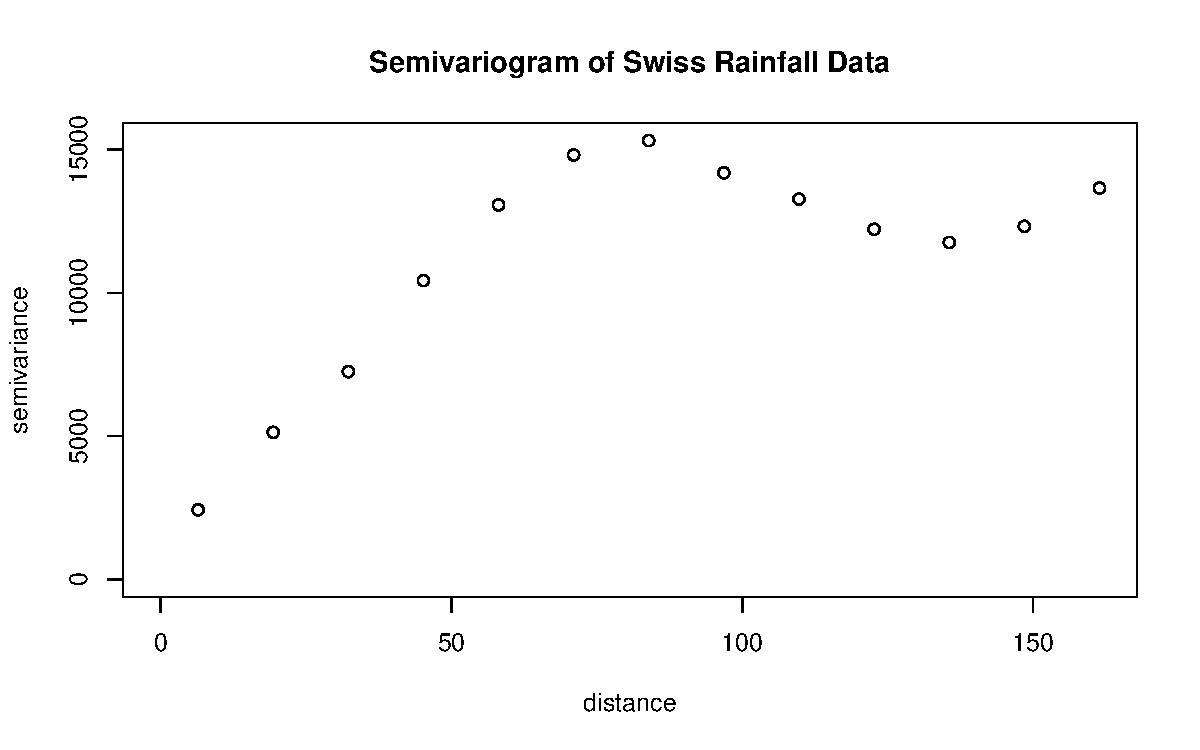
\includegraphics[width=\maxwidth]{figure/rainfall} 

\end{knitrout}

\item
Do you think the residuals from the linear model regressing the variable altitude (called elevation in class) on rainfall exhibit spatial dependence? Briefly explain and provide a graphic to support your answer.

\textsf{
Yes, according to the residuals variogram, the residuals exhibit evidence of spatial dependence. That is because the trend in the variogram is similar to the one in the previous problem. 
}
\begin{knitrout}
\definecolor{shadecolor}{rgb}{0.969, 0.969, 0.969}\color{fgcolor}
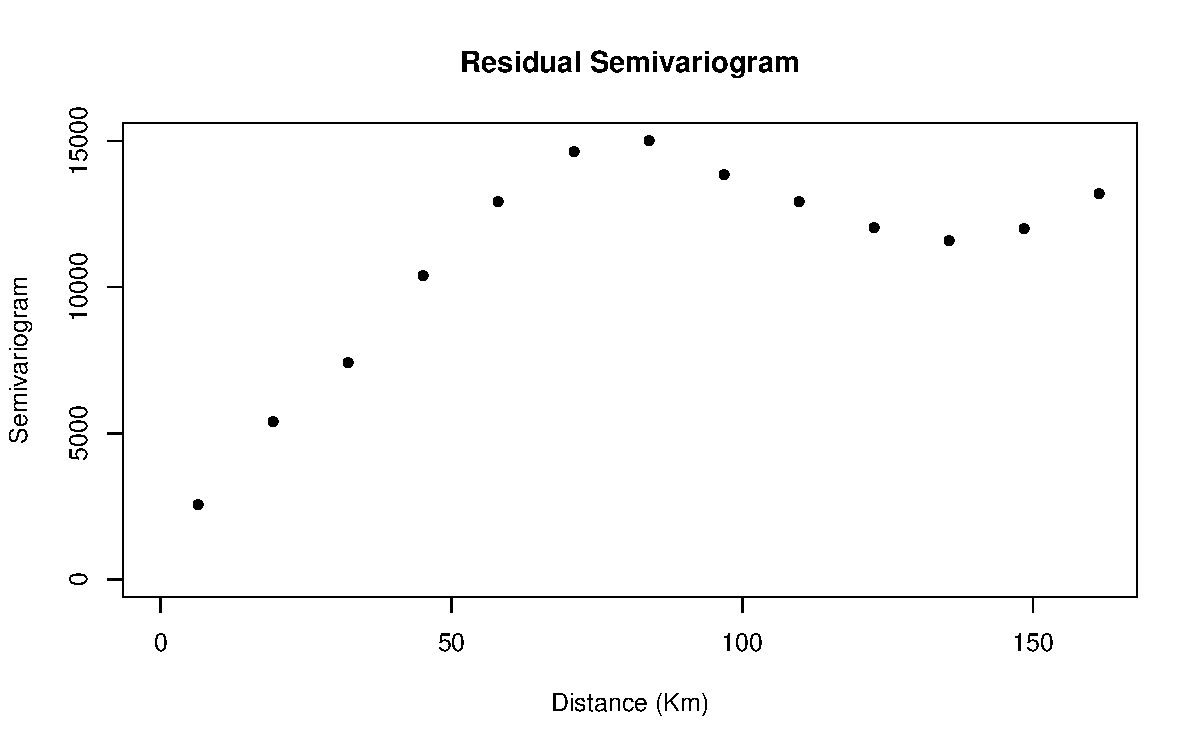
\includegraphics[width=\maxwidth]{figure/residual} 

\end{knitrout}

\item
Do you think altitude accounted for much of the spatial variation in the rainfall measurements? Briefly explain.

\textsf{
If altitude accounted for much of the spatial variation of the rainfall, then the linear regression would control for that variation and the residuals would have ``perceptibly'' less change in spatial variation  (a flatter variogram curve) than the rainfall variogram. 
It is observed, however, that the variograms of residuals and rainfall show nearly the same values for the same distances. 
This means that the spatial dependence of elevation does not explain much of the spatial variation of rainfall.  
}
\item
Using the eyefit command suggest values for the range, partial sill, and nugget for an exponential semivariogram model drawn to the rainfall semivariogram estimates. Provide the graph of the rainfall semivariogram estimates with the drawn in exponential function line as well. Note for Mac users: The eyefit command requires certain software and other packages to be downloaded to work properly on Macs and even then we have had several issues in years past. Alternatively just ‘eyeball” a set of parameter estimates and hand that in as your answer here. And you should do this all the time when code I provide suggests using the eyefit command.



\textsf{
\begin{itemize}
\item
Total Sill -- 14500
\item
Nugget -- 2000
\item
Partial Sill -- 12500
\item
Range -- 35
\end{itemize}
}
\begin{knitrout}
\definecolor{shadecolor}{rgb}{0.969, 0.969, 0.969}\color{fgcolor}
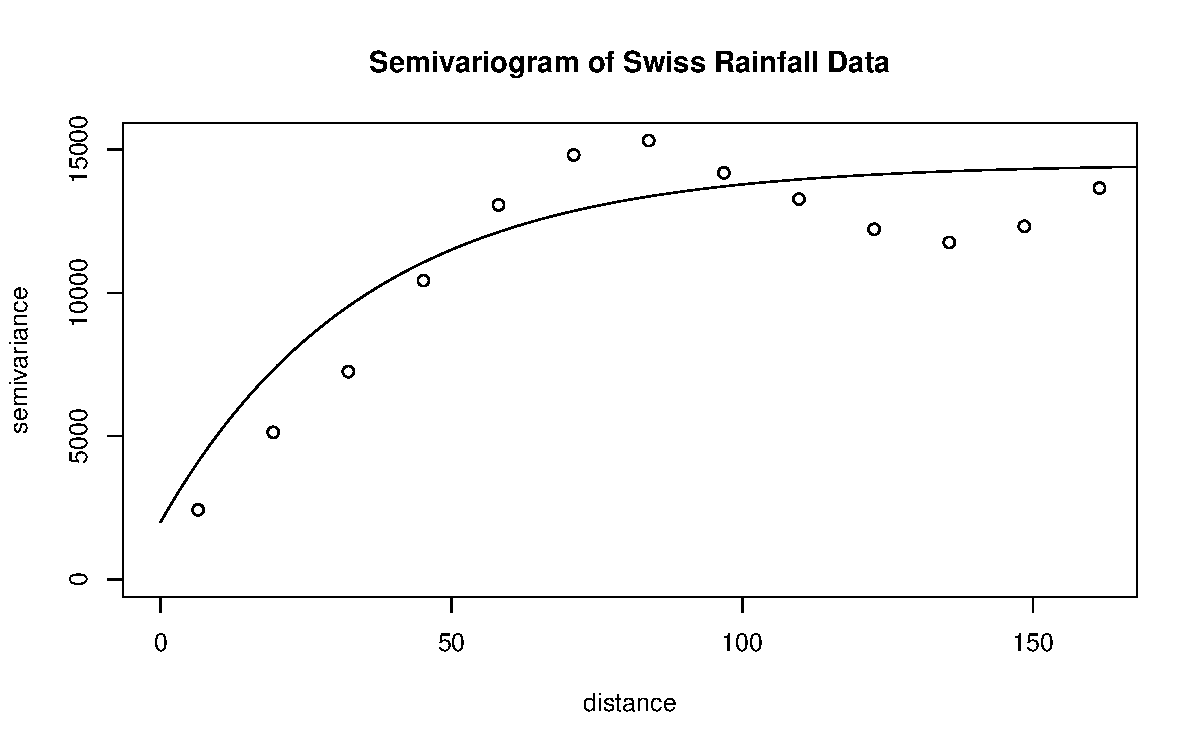
\includegraphics[width=\maxwidth]{figure/better} 

\end{knitrout}




\subsubsection*{Naive attempt}
From tinkering with the values, it appears that \textit{range} is actually the inflection point for the exponential. From the class notes, I thought that the range was the $x$ value about where the curve starts to flatten out (I realize now that that is the rough definition of ``inflection point''). The range was the most important parameter to get right for the curve. For the sake of history, I am leaving in my first attempt at this problem.



\textsf{
\begin{itemize}
\item
Total Sill -- 15000
\item
Nugget -- 1000
\item
Partial Sill -- 14000
\item
Range -- 75
\end{itemize}
}

\begin{knitrout}
\definecolor{shadecolor}{rgb}{0.969, 0.969, 0.969}\color{fgcolor}
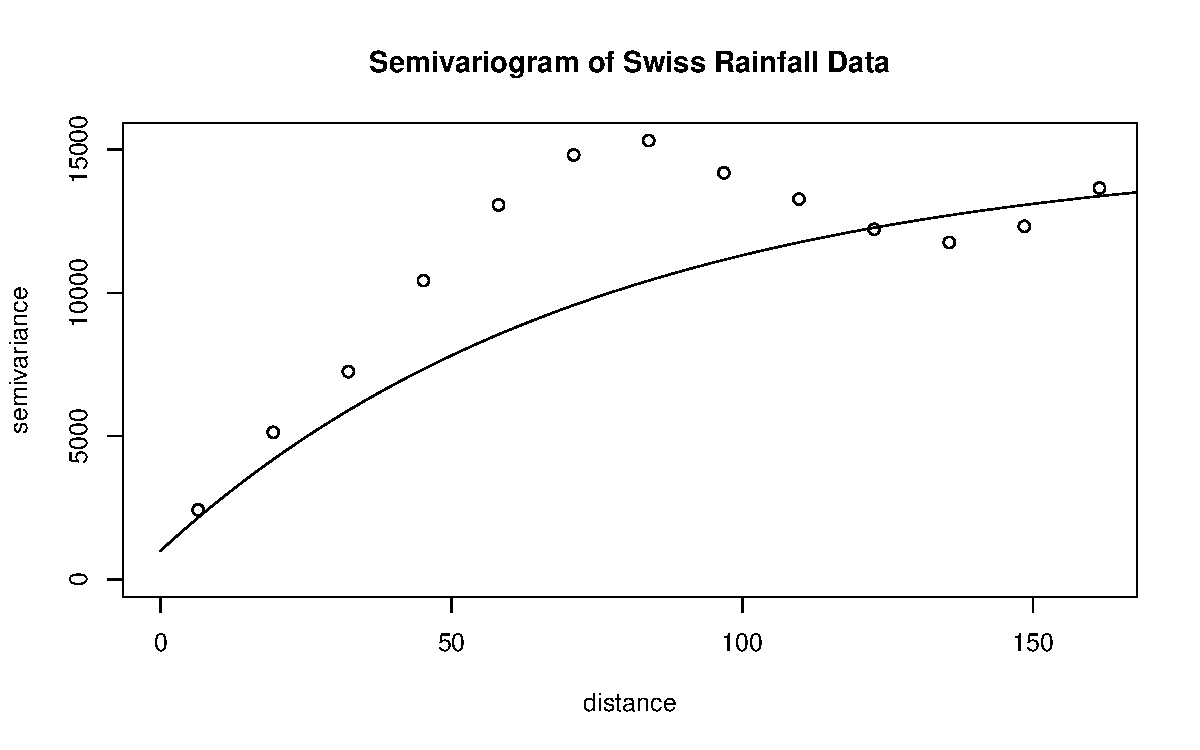
\includegraphics[width=\maxwidth]{figure/linefitexp} 

\end{knitrout}

\end{enumerate}
\subsection*{Wolfcamp Aquifer Data}
\begin{enumerate}[e.]
\item
Do you think the pressure measurements exhibit spatial dependence? Briefly explain and provide a graphic to support your answer.

\textsf{
Yes, the pressure measurements exhibit spatial dependence. See the variogram of pressure measurements. As distance increases between measurements, the variation increases. This is a strong indication of spatial dependence (nearer measurements are more similar than ones farther away).
}

\begin{knitrout}
\definecolor{shadecolor}{rgb}{0.969, 0.969, 0.969}\color{fgcolor}
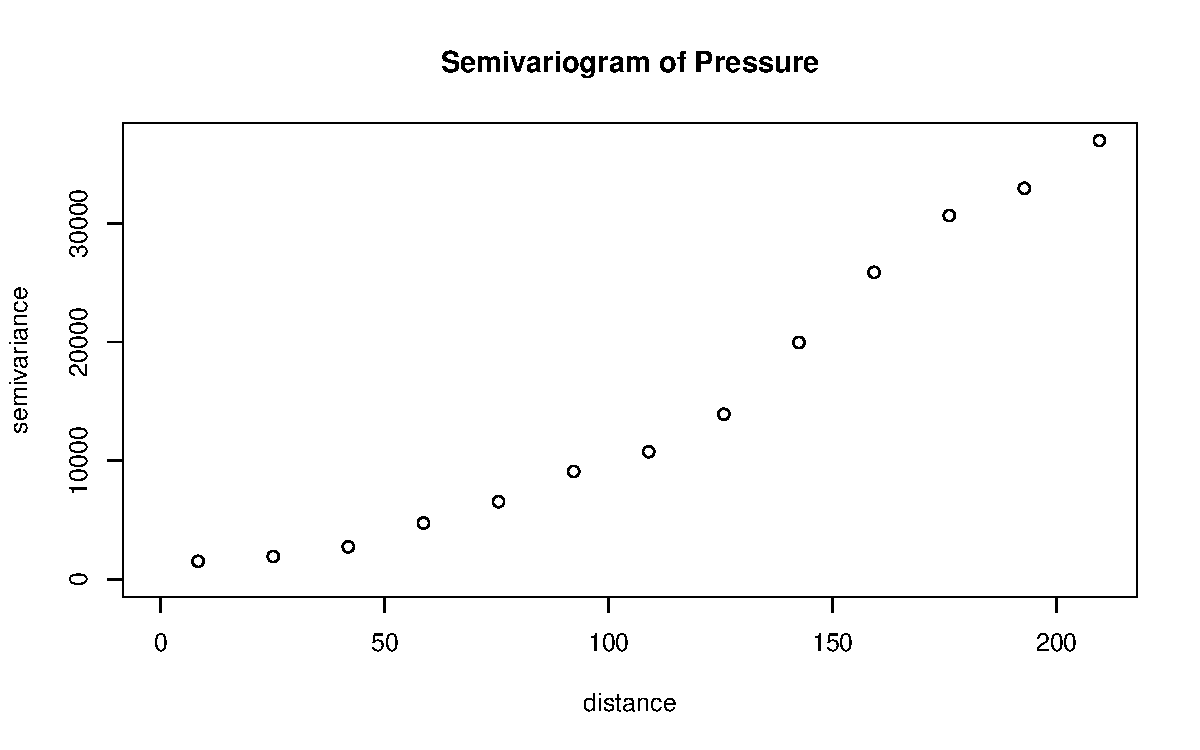
\includegraphics[width=\maxwidth]{figure/wolfcamp} 

\end{knitrout}


\item
Do you think there is any evidence for a large scale spatial trend as a function of either or both coordinates? Briefly explain and provide a graphic to support your answer.

\textsf{
There is some evidence. See the plots ``\texttt{Data vs X coord}'' and ``\texttt{Y coord vs data}.'' These two plots are both roughly linear. Hence, one might be able to quantify the following: ``given a unit change in the $X$ coordinate, the data typically change by $m_X$.'' The same is true for the $Y$ coordinate. This is evidence for a large scale spatial trend as a function of both coordinates.
}
\begin{knitrout}
\definecolor{shadecolor}{rgb}{0.969, 0.969, 0.969}\color{fgcolor}
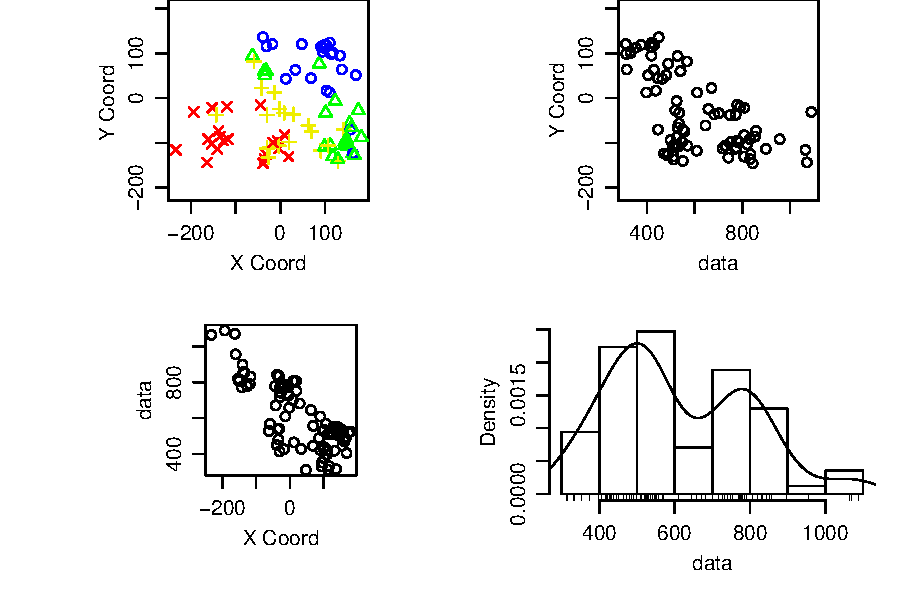
\includegraphics[width=\maxwidth]{figure/wolfcamp2} 

\end{knitrout}

\end{enumerate}
\subsection*{Previous Years R Demo}
The files called \texttt{IntroR 2012.pdf, Lab1 2012.R}, and \texttt{Attribute Ozone2007.csv} in the zipped folder \texttt{Previous Years R Demo} were files used in a previous year R demonstration during the first lab. Look through the pdf slides and run through the R demo for another introduction to R. Nothing is to be handed in for this.

\textsf{Done.}


\end{document}
